% CAPÍTULO 4 — DESENVOLVIMENTO E RESULTADOS

\chapter{DESENVOLVIMENTO E RESULTADOS}
\label{cap:desenvolvimento}

Este capítulo descreve o sistema efetivamente implementado a partir do planejamento apresentado no Capítulo~\ref{cap:metodos}. São apresentados a arquitetura adotada no \textit{backend} e no \textit{frontend}, o modelo de dados, os mecanismos de segurança, a interface de programação disponibilizada, as funcionalidades desenvolvidas, a verificação do atendimento aos requisitos e as limitações identificadas.

\section{Visão Geral da Solução}

O SIGEI foi construído como uma aplicação web composta por três elementos independentes: uma API REST desenvolvida em Java com Spring Boot, uma aplicação de página única (SPA) desenvolvida em Angular e um banco de dados relacional PostgreSQL. As fotografias das escolas são armazenadas em um serviço externo de hospedagem de imagens, o Cloudinary, e o banco de dados guarda apenas o endereço de cada imagem.

A aplicação oferece dois modos de acesso. O primeiro é um mapa público, acessível sem autenticação, que apresenta a localização georreferenciada das escolas indígenas do Acre. O segundo é uma área administrativa, restrita a usuários autenticados, na qual são realizados os cadastros, a manutenção do histórico anual das escolas e a consulta aos indicadores consolidados.

Em relação ao planejamento inicial, algumas decisões tecnológicas foram revistas durante a implementação. O \textit{backend} foi desenvolvido em Java 21 com Spring Boot 4, e o \textit{frontend} em Angular 21. O Leaflet passou a ser utilizado diretamente, sem o pacote intermediário \texttt{ngx-leaflet}, o que simplificou a integração com os componentes independentes (\textit{standalone}) do Angular.

\section{Arquitetura Implementada}

\subsection{\textit{Backend}}

O \textit{backend} segue a arquitetura em camadas descrita no Capítulo~\ref{cap:metodos}, na qual cada requisição percorre o fluxo controlador, serviço e repositório \cite{pressman2016}. Os controladores recebem as requisições HTTP e validam os dados de entrada; os serviços concentram as regras de negócio e delimitam as transações; os repositórios, baseados no Spring Data JPA, realizam o acesso ao banco de dados \cite{walls2019}. A conversão entre entidades e objetos de transferência de dados (DTOs) é feita por interfaces do MapStruct, que geram o código de conversão em tempo de compilação. Assim, as entidades JPA nunca são expostas diretamente na API. O Quadro~\ref{qua:pacotes} resume a organização dos pacotes.

\begin{longtable}{p{3.5cm}p{10cm}}
\caption{Organização dos pacotes do \textit{backend}}
\label{qua:pacotes} \\
\toprule
\textbf{Pacote} & \textbf{Responsabilidade} \\
\midrule
\endfirsthead
\toprule
\textbf{Pacote} & \textbf{Responsabilidade} \\
\midrule
\endhead
\midrule
\multicolumn{2}{r}{\small\textit{continua na próxima página}} \\
\endfoot
\bottomrule
\endlastfoot
\texttt{controllers}  & Definição das rotas HTTP, validação da entrada e montagem das respostas. \\[3pt]
\texttt{service}      & Regras de negócio, transações, autenticação, armazenamento de imagens e importação de planilhas. \\[3pt]
\texttt{repository}   & Interfaces Spring Data JPA, consultas personalizadas e agregações dos indicadores. \\[3pt]
\texttt{models}       & Entidades JPA e enumerações do domínio. \\[3pt]
\texttt{dto}          & Contratos de entrada (\textit{request}) e de saída (\textit{response}) da API. \\[3pt]
\texttt{mappers}      & Conversão entre entidades e DTOs com MapStruct. \\[3pt]
\texttt{config}       & Segurança, inicialização de dados e integração com o Cloudinary. \\[3pt]
\texttt{exceptions}   & Exceções da aplicação e tratamento global de erros HTTP. \\[3pt]
\texttt{utils}        & Leitura de planilhas Excel, normalização de coordenadas e contadores de importação. \\
\end{longtable}
\fonte{Euzébio do Nascimento Oliveira Neto (2026)}

O tratamento de erros é centralizado em um componente anotado com \texttt{@RestControllerAdvice}, que converte as exceções em respostas HTTP padronizadas: 400 para dados inválidos, 404 para recursos inexistentes, 409 para violações de integridade referencial e 503 quando o serviço de armazenamento de imagens não está configurado.

\subsection{\textit{Frontend}}

O \textit{frontend} foi construído com componentes independentes (\textit{standalone components}) do Angular, dispensando a declaração de módulos \cite{angular2023}. O código foi organizado em quatro áreas:

\begin{alineas}
  \item \textbf{\texttt{core}:} serviço de autenticação, interceptador HTTP e \textit{guards} de rota;
  \item \textbf{\texttt{domains}:} serviços de acesso à API e modelos de dados, agrupados pelos domínios escolas, territórios e usuários;
  \item \textbf{\texttt{features}:} telas da aplicação, agrupadas em mapa público, autenticação e área administrativa;
  \item \textbf{\texttt{shared}:} componentes visuais reutilizáveis, como cabeçalho e janelas de confirmação.
\end{alineas}

Todas as telas são carregadas sob demanda (\textit{lazy loading}): o navegador baixa o código de cada página apenas quando ela é acessada, o que reduz o tempo de carregamento inicial do mapa público. A aplicação também utiliza a detecção de mudanças sem a biblioteca Zone.js, recurso disponível nas versões recentes do Angular. A estilização foi feita com o \textit{framework} de CSS utilitário Tailwind CSS, que permitiu construir uma interface responsiva a partir de classes aplicadas diretamente nos \textit{templates} \cite{freeman2019}.

\subsection{Implantação}

Tanto o \textit{backend} quanto o \textit{frontend} possuem arquivos \texttt{Dockerfile} e \texttt{docker-compose}, o que permite executar o sistema completo em contêineres. O contêiner do \textit{backend} é acompanhado de um contêiner PostgreSQL com volume persistente. O do \textit{frontend} utiliza o servidor Nginx, configurado para redirecionar as rotas da SPA para o arquivo \texttt{index.html}, aplicar compressão e cabeçalhos de segurança e encaminhar as chamadas à API. As configurações sensíveis, como credenciais do banco de dados, segredo de assinatura dos \textit{tokens} e chaves do Cloudinary, são fornecidas por variáveis de ambiente e não são versionadas no repositório.

% TODO: inserir diagrama de implantação (navegador → Nginx/Angular → API Spring Boot → PostgreSQL e Cloudinary)
% \begin{figure}[H]
% \centering
% \includegraphics[width=0.85\textwidth]{imagens/diagrama-implantacao.png}
% \caption{Diagrama de implantação do SIGEI}
% \fonte{Euzébio do Nascimento Oliveira Neto (2026)}
% \label{fig:implantacao}
% \end{figure}

\section{Modelo de Dados}

O modelo de dados implementado é composto por treze entidades persistidas pelo Hibernate \cite{bauer2015}. As entidades territoriais formam uma hierarquia: \texttt{Municipio} contém \texttt{TerraIndigena}; \texttt{Aldeia} pertence a uma terra indígena e está associada a um \texttt{Povo}; \texttt{Escola} está localizada em uma aldeia. A entidade \texttt{Usuario} armazena as credenciais e o perfil de acesso.

A principal decisão de modelagem foi separar os dados permanentes da escola dos dados que variam a cada ano. A entidade \texttt{Escola} guarda apenas os atributos estáveis: código INEP, nome, tipo de unidade (sede ou anexo) e escola-sede, quando se tratar de anexo. As informações anuais ficam na entidade \texttt{RegistroAnual}, que associa uma escola a um \texttt{AnoReferencia}. Uma restrição de unicidade sobre o par escola e ano impede registros duplicados. Cada registro anual possui:

\begin{alineas}
  \item uma \texttt{EquipeEscola}, que indica a presença de professor responsável, equipe gestora, merendeira, zeladora e barqueiro, além da necessidade de transporte;
  \item uma \texttt{InfraestruturaEscola}, com ano de construção, número de salas, coordenadas geográficas, situação de funcionamento, tipo de acesso, abastecimento de água, energia, internet, existência de prédio e fotografia;
  \item um conjunto de \texttt{MatriculaNivel}, com as matrículas por nível de ensino e por sexo;
  \item um conjunto de \texttt{MatriculaSerie}, com as matrículas por ano ou série, incluindo os ciclos da Educação de Jovens e Adultos.
\end{alineas}

Essa estrutura preserva o histórico de cada unidade escolar: a atualização dos dados de um ano não altera os registros dos anos anteriores. Como as coordenadas ficam na infraestrutura anual, e não na escola, eventuais mudanças de local de funcionamento também são preservadas no histórico. Os relacionamentos entre o registro anual e seus dependentes utilizam exclusão em cascata, de modo que a remoção de um registro elimina também a equipe, a infraestrutura e as matrículas correspondentes.

% TODO: substituir pelo diagrama ER atualizado (13 entidades). O arquivo sigei-backend/docs/MODELO_ER.md
% contém o diagrama em Mermaid gerado a partir das entidades JPA.
% \begin{figure}[H]
% \centering
% \includegraphics[width=0.95\textwidth]{imagens/modelo-er-implementado.png}
% \caption{Modelo entidade-relacionamento implementado}
% \fonte{Euzébio do Nascimento Oliveira Neto (2026)}
% \label{fig:erimplementado}
% \end{figure}

O esquema do banco é gerado e atualizado pelo Hibernate a partir das entidades, conforme a propriedade \texttt{spring.jpa.hibernate.ddl-auto}. As coordenadas geográficas são armazenadas como números de precisão dupla, conforme previsto no planejamento.

\section{Segurança e Controle de Acesso}

A autenticação foi implementada com o Spring Security em modo sem estado (\textit{stateless}), com \textit{tokens} JWT (\textit{JSON Web Token}). O fluxo ocorre da seguinte forma:

\begin{alineas}
  \item o usuário informa e-mail e senha na tela de \textit{login};
  \item o \textit{backend} verifica se o usuário está ativo e compara a senha com o valor armazenado, cifrado com o algoritmo BCrypt;
  \item em caso de sucesso, é emitido um \textit{token} assinado com validade padrão de 24 horas, contendo a identificação e o perfil do usuário;
  \item o \textit{frontend} armazena o \textit{token} e o envia no cabeçalho \texttt{Authorization} de cada requisição por meio de um interceptador HTTP;
  \item a cada requisição, um filtro do \textit{backend} valida o \textit{token} e consulta novamente o cadastro do usuário, de modo que a desativação de uma conta tem efeito imediato.
\end{alineas}

Foram definidos dois perfis de acesso, correspondentes aos atores do diagrama de casos de uso (Figura~\ref{fig:casosdeuso}): \texttt{ADMIN}, equivalente ao Gestor, e \texttt{USUARIO}, equivalente ao Consulente. O Quadro~\ref{qua:permissoes} apresenta as regras de autorização aplicadas.

\begin{longtable}{p{6cm}p{7.5cm}}
\caption{Regras de autorização da API}
\label{qua:permissoes} \\
\toprule
\textbf{Requisição} & \textbf{Acesso} \\
\midrule
\endfirsthead
\toprule
\textbf{Requisição} & \textbf{Acesso} \\
\midrule
\endhead
\midrule
\multicolumn{2}{r}{\small\textit{continua na próxima página}} \\
\endfoot
\bottomrule
\endlastfoot
\textit{Login}, verificação de saúde e documentação da API & Público \\[3pt]
Consulta às infraestruturas (dados do mapa)              & Público \\[3pt]
Alteração da própria senha                                 & Qualquer usuário autenticado \\[3pt]
Demais consultas (\texttt{GET})                            & Perfis \texttt{ADMIN} e \texttt{USUARIO} \\[3pt]
Inclusões, alterações e exclusões                          & Somente \texttt{ADMIN} \\
\end{longtable}
\fonte{Euzébio do Nascimento Oliveira Neto (2026)}

O administrador inicial é criado automaticamente na primeira execução do sistema com a troca de senha marcada como obrigatória. Enquanto a senha não é alterada, o \textit{token} emitido concede apenas a permissão de trocá-la, e o \textit{frontend} redireciona o usuário para a tela correspondente. O mesmo ocorre com os usuários cadastrados por um administrador.

No \textit{frontend}, \textit{guards} de rota impedem a navegação para páginas não permitidas ao perfil do usuário e ocultam os botões de edição para o perfil \texttt{USUARIO}. Essa verificação serve à usabilidade. A garantia efetiva de acesso é feita no \textit{backend}, que rejeita com os códigos 401 ou 403 qualquer requisição não autorizada, independentemente da interface utilizada. O compartilhamento de recursos entre origens (CORS) é restrito às origens configuradas para o \textit{frontend}.

\section{Interface de Programação da Aplicação}

A API segue o estilo arquitetural REST \cite{fielding2000}, com recursos identificados por URIs, operações expressas pelos verbos HTTP e representação em JSON \cite{richardson2013}. O Quadro~\ref{qua:endpoints} resume os recursos disponibilizados.

\begin{longtable}{p{4cm}p{9.5cm}}
\caption{Recursos da API REST do SIGEI}
\label{qua:endpoints} \\
\toprule
\textbf{Recurso} & \textbf{Operações} \\
\midrule
\endfirsthead
\toprule
\textbf{Recurso} & \textbf{Operações} \\
\midrule
\endhead
\midrule
\multicolumn{2}{r}{\small\textit{continua na próxima página}} \\
\endfoot
\bottomrule
\endlastfoot
\texttt{/municipio}          & Cadastro e consulta; estatísticas por município. \\[3pt]
\texttt{/terra}              & Cadastro e consulta de terras indígenas; estatísticas. \\[3pt]
\texttt{/aldeia}, \texttt{/povo} & Cadastro e consulta. \\[3pt]
\texttt{/escola}             & Cadastro e consulta; detalhe da escola com o registro anual mais recente. \\[3pt]
\texttt{/anos}               & Cadastro dos anos de referência. \\[3pt]
\texttt{/registroAnual}      & Cadastro; consulta por ano, por escola e ano, e histórico de uma escola em um intervalo de anos. \\[3pt]
\texttt{/equipe}             & Inclusão e alteração da equipe de um registro anual. \\[3pt]
\texttt{/infraestrutura}     & Cadastro e consulta; consulta por ano; envio de fotografia. \\[3pt]
\texttt{/matriculaNivel}, \texttt{/matriculaSerie} & Cadastro das matrículas de um registro anual. \\[3pt]
\texttt{/atualizacao-anual}  & Abertura de um novo ano de referência. \\[3pt]
\texttt{/importacoes}        & Importação de planilhas de infraestrutura e de matrículas. \\[3pt]
\texttt{/dashboard}          & Indicadores consolidados, com ano opcional. \\[3pt]
\texttt{/usuario}            & Cadastro e consulta de usuários. \\[3pt]
\texttt{/auth}               & \textit{Login} e alteração de senha. \\
\end{longtable}
\fonte{Euzébio do Nascimento Oliveira Neto (2026)}

A API é documentada automaticamente com a especificação OpenAPI, gerada pela biblioteca Springdoc a partir de anotações nos controladores. A documentação interativa fica disponível na interface Swagger UI, que permite consultar os contratos de entrada e saída e testar as operações diretamente pelo navegador.

\section{Funcionalidades Desenvolvidas}

\subsection{Mapa Público Interativo}

O mapa público é a página inicial do sistema e não exige autenticação. Ele foi desenvolvido com a biblioteca Leaflet \cite{leaflet2023} e apresenta um marcador para cada escola com coordenadas cadastradas, posicionado sobre o território do Acre. A cor do marcador indica a situação da unidade: verde para escolas em funcionamento e vermelho para escolas paralisadas. Essa codificação permite identificar visualmente a distribuição espacial das unidades que demandam atenção \cite{longley2013}.

O usuário pode alternar entre quatro camadas de fundo (mapa padrão do OpenStreetMap, imagem de satélite, relevo e tema escuro), pesquisar escolas por nome ou código INEP e aplicar filtros por situação, tipo de acesso (terrestre, fluvial, aéreo ou misto), disponibilidade de internet e existência de prédio. Ao selecionar uma escola, o mapa é centralizado sobre ela e exibe uma janela com fotografia, código INEP, situação, tipo de acesso e indicadores de infraestrutura.

% TODO: inserir captura de tela do mapa público
% \begin{figure}[H]
% \centering
% 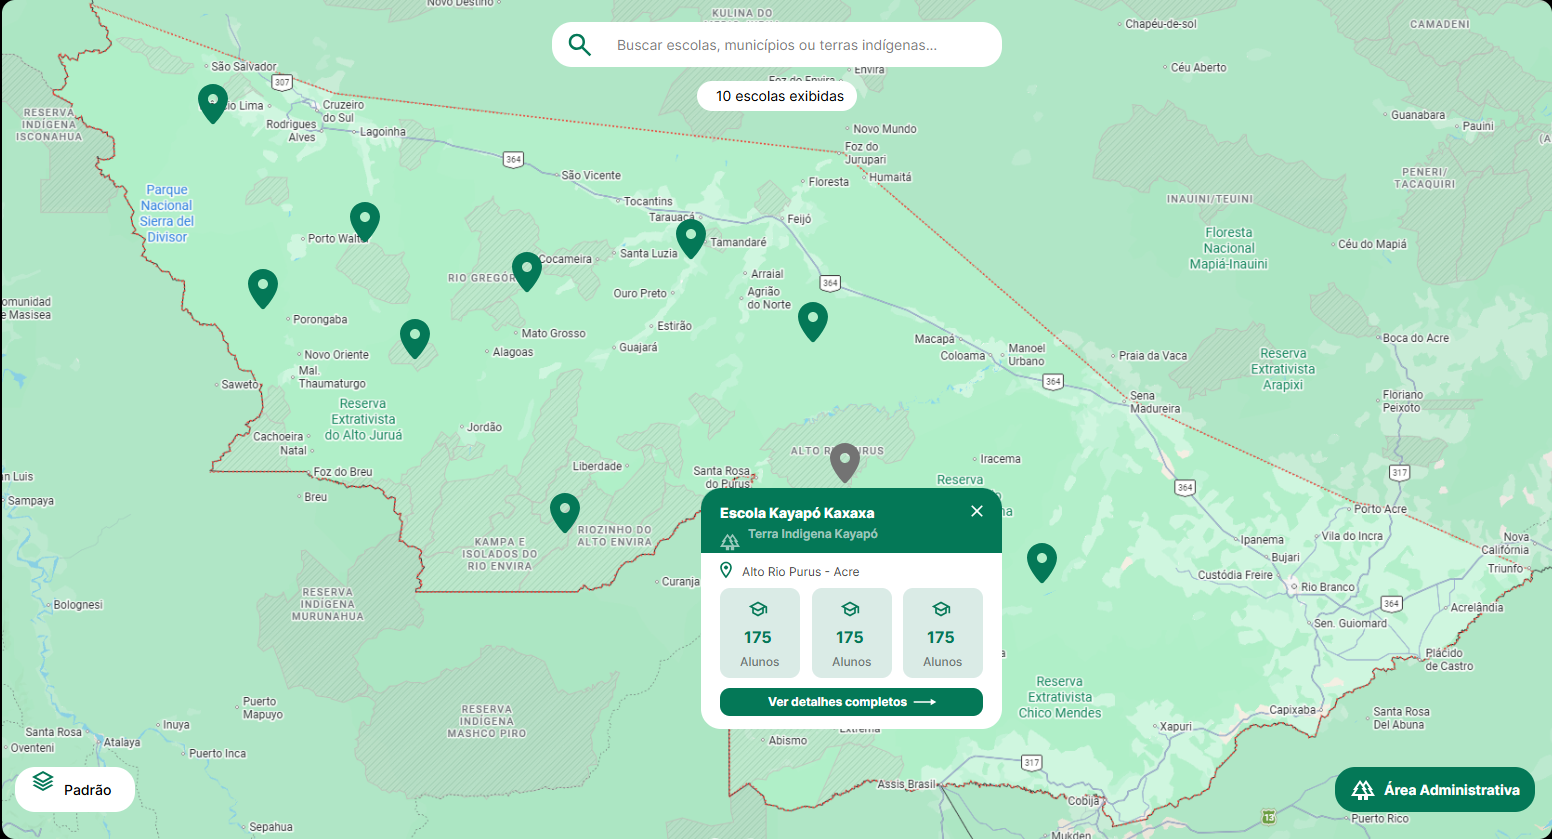
\includegraphics[width=0.95\textwidth]{imagens/tela-mapa.png}
% \caption{Mapa público do SIGEI}
% \fonte{Euzébio do Nascimento Oliveira Neto (2026)}
% \label{fig:telamapa}
% \end{figure}

\subsection{Painel de Indicadores}

Após a autenticação, o usuário é direcionado a um painel (\textit{dashboard}) que consolida as informações de um ano de referência, por padrão o mais recente. O painel apresenta:

\begin{alineas}
  \item totais de escolas, matrículas, municípios e terras indígenas;
  \item evolução do número de matrículas e de escolas ao longo dos anos cadastrados;
  \item distribuição das matrículas por nível de ensino;
  \item percentual de escolas com internet, energia elétrica e prédio próprio;
  \item quantidade de escolas por município e por situação de funcionamento.
\end{alineas}

Os indicadores são calculados no banco de dados por consultas de agregação, e o \textit{frontend} apenas recebe os valores consolidados. O painel atende ao objetivo de disponibilizar informações gerenciais aos gestores da SEE/AC.

% TODO: inserir captura de tela do dashboard
% \begin{figure}[H]
% \centering
% \includegraphics[width=0.95\textwidth]{imagens/tela-dashboard.png}
% \caption{Painel de indicadores}
% \fonte{Euzébio do Nascimento Oliveira Neto (2026)}
% \label{fig:teladashboard}
% \end{figure}

\subsection{Cadastros Territoriais}

A área administrativa oferece telas de listagem, pesquisa e manutenção para terras indígenas, aldeias e povos. Todas as exclusões exigem confirmação prévia. Os municípios do Acre são cadastrados automaticamente pelo sistema na inicialização, e a tela correspondente apresenta, para cada município, a quantidade de terras indígenas, aldeias e escolas associadas.

\subsection{Cadastro de Escolas}

Por envolver muitas informações, o cadastro de escolas foi dividido em sete etapas sequenciais, cada uma validada antes do avanço para a seguinte:

\begin{alineas}
  \item dados da escola: código INEP, nome, tipo de unidade, aldeia e, para anexos, a escola-sede;
  \item registro anual: ano de referência, rede de ensino e local de funcionamento;
  \item equipe escolar;
  \item infraestrutura, com coordenadas geográficas e envio opcional de fotografia;
  \item matrículas por nível de ensino (Educação Infantil, Ensino Fundamental -- anos iniciais e finais, Ensino Médio, EJA e AEE), separadas por sexo;
  \item matrículas por ano ou série, do 1.º ano do Ensino Fundamental à 3.ª série do Ensino Médio, além dos ciclos da EJA;
  \item revisão dos dados antes da gravação.
\end{alineas}

Os totais de matrículas são calculados automaticamente pela interface à medida que as quantidades são informadas. A mesma tela é utilizada para a edição, quando carrega os dados já cadastrados da escola.

% TODO: inserir captura de tela de uma etapa do cadastro de escolas
% \begin{figure}[H]
% \centering
% \includegraphics[width=0.95\textwidth]{imagens/tela-cadastro-escola.png}
% \caption{Cadastro de escolas em etapas}
% \fonte{Euzébio do Nascimento Oliveira Neto (2026)}
% \label{fig:telacadastroescola}
% \end{figure}

\subsection{Histórico Anual e Abertura de Novo Ano}

A tela de histórico permite consultar os registros de duas formas: todos os registros de um ano ou a evolução de uma escola específica em um intervalo de anos. A partir dela, o administrador pode editar os dados de um ano específico ou cadastrar retroativamente um ano anterior, sem afetar os demais registros da escola.

Para a virada do ano letivo, foi implementada a operação de abertura de novo ano. Ela cria o ano de referência seguinte ao mais recente e, para cada escola, gera um novo registro anual copiando rede, local de funcionamento, equipe, infraestrutura e matrículas do último registro existente. A operação é executada em uma única transação no banco de dados. O gestor passa então a atualizar apenas as informações que mudaram, sem recadastrar as escolas.

\subsection{Carga Inicial e Importação de Planilhas}

Para aproveitar os dados já existentes na SEE/AC, que antes estavam dispersos em planilhas eletrônicas, foi desenvolvido um módulo de importação com a biblioteca Apache POI. Ele lê a planilha de infraestrutura e a planilha de matrículas do censo escolar, normaliza os nomes, converte as coordenadas geográficas e identifica as escolas. As terras indígenas, povos, aldeias e escolas ainda não cadastrados são criados, e os registros anuais correspondentes são criados ou atualizados. Ao final, informa a quantidade de linhas processadas e os erros encontrados.

Na primeira execução do sistema com o banco de dados vazio, essa importação é realizada automaticamente. Assim, o sistema já é disponibilizado com os dados das escolas indígenas carregados. A importação também está disponível pela API para uso posterior.

\subsection{Gestão de Usuários e Preferências}

Os administradores podem cadastrar, editar, ativar e desativar usuários e definir o perfil de acesso de cada um. Cada usuário pode ainda ajustar preferências de exibição do mapa, como a camada de fundo padrão, a abertura das janelas ao passar o cursor e a exibição de fotografias. Essas preferências são armazenadas no próprio navegador.

\section{Atendimento aos Requisitos}

O Quadro~\ref{qua:atendimentorf} relaciona os requisitos funcionais apresentados no Quadro~\ref{qua:rf} às funcionalidades implementadas.

\begin{longtable}{p{1.5cm}p{3cm}p{2.2cm}p{6.8cm}}
\caption{Atendimento aos requisitos funcionais}
\label{qua:atendimentorf} \\
\toprule
\textbf{Código} & \textbf{Requisito} & \textbf{Situação} & \textbf{Implementação} \\
\midrule
\endfirsthead
\toprule
\textbf{Código} & \textbf{Requisito} & \textbf{Situação} & \textbf{Implementação} \\
\midrule
\endhead
\midrule
\multicolumn{4}{r}{\small\textit{continua na próxima página}} \\
\endfoot
\bottomrule
\endlastfoot
RF01 & Cadastrar escola          & Atendido & Cadastro em sete etapas, com dados anuais, infraestrutura, fotografia e matrículas. \\[3pt]
RF02 & Editar escola             & Atendido & Edição dos dados permanentes e de qualquer ano do histórico. \\[3pt]
RF03 & Excluir escola            & Atendido & Exclusão com confirmação prévia. \\[3pt]
RF04 & Visualizar no mapa        & Atendido & Mapa Leaflet com marcadores diferenciados por situação. \\[3pt]
RF05 & Gerenciar aldeias         & Atendido & Cadastro, edição, consulta e exclusão, vinculados à terra indígena e ao povo. \\[3pt]
RF06 & Gerenciar municípios      & Atendido & Carga automática dos municípios do Acre e consulta com estatísticas; API com operações completas. \\[3pt]
RF07 & Gerenciar terras indígenas & Atendido & Cadastro, edição, consulta e exclusão. \\[3pt]
RF08 & Gerar relatórios          & Parcial  & Indicadores consolidados no painel; exportação de relatórios em arquivo não implementada. \\[3pt]
RF09 & Registrar matrículas      & Atendido & Matrículas por nível e por série, por sexo, em cada ano de referência. \\[3pt]
RF10 & Consultar mapa interativo & Atendido & Busca, filtros e janela de informações por escola. \\
\end{longtable}
\fonte{Euzébio do Nascimento Oliveira Neto (2026)}

Quanto aos requisitos não funcionais, a interface foi construída com classes responsivas do Tailwind CSS e se adapta a telas de dispositivos móveis (RNF01). O sistema é acessado por navegador, sem instalação de \textit{software} adicional (RNF02). O controle de acesso é garantido pela autenticação JWT e pelos perfis descritos na seção anterior (RNF03). A integridade dos dados é assegurada por chaves estrangeiras, restrições de unicidade e validações com \textit{Bean Validation} na camada de aplicação (RNF06). O desempenho do mapa (RNF04) e a usabilidade (RNF05) não foram submetidos a medições ou testes formais com usuários, o que fica registrado como trabalho futuro.

\section{Testes}

A verificação do \textit{backend} foi realizada com testes automatizados escritos com JUnit 5 e Mockito, organizados em 27 classes de teste que espelham os pacotes da aplicação \cite{sommerville2019}. Os testes de serviço isolam as regras de negócio por meio de objetos simulados (\textit{mocks}) dos repositórios. Os testes de repositório utilizam a anotação \texttt{@DataJpaTest} com um banco de dados H2 em memória, verificando os mapeamentos, as consultas personalizadas e as agregações do painel de indicadores. Também foram testados o inicializador de municípios e o histórico anual das escolas.

Além dos testes automatizados, as rotas da API foram verificadas manualmente com uma coleção de requisições da ferramenta Bruno, e as telas do \textit{frontend} foram validadas por testes funcionais manuais durante cada incremento de desenvolvimento. O \textit{frontend} possui o executor de testes Vitest configurado, mas ainda não conta com testes automatizados.

\section{Limitações e Trabalhos Futuros}

Durante o desenvolvimento, foram identificadas as seguintes limitações, que orientam a continuidade do projeto:

\begin{alineas}
  \item a exportação de relatórios em formatos como PDF ou planilha ainda não foi implementada;
  \item o módulo de importação foi construído para o leiaute das planilhas disponibilizadas pela SEE/AC, com colunas e ano de referência fixos, e precisa ser generalizado para cargas de anos futuros;
  \item o cadastro de uma escola é gravado por uma sequência de requisições à API, e não por uma única transação, de modo que uma falha intermediária pode deixar o cadastro incompleto até nova gravação;
  \item não há renovação automática do \textit{token} de acesso; após o período de validade, o usuário precisa se autenticar novamente;
  \item o \textit{frontend} não possui testes automatizados, e não foram realizadas avaliações formais de desempenho e de usabilidade com os gestores da SEE/AC;
  \item o esquema do banco de dados é mantido pelo Hibernate, e a adoção de uma ferramenta de versionamento de esquema, como Flyway, é recomendável antes do uso em produção.
\end{alineas}
